\documentclass[10pt,letterpaper]{article}
\usepackage[margin=0.75in]{geometry}
\usepackage{listings}
\usepackage{color}
\usepackage{longtable}
\usepackage{tabu}
\usepackage{pgfplots}

\definecolor{dkgreen}{rgb}{0,0.6,0}
\definecolor{gray}{rgb}{0.5,0.5,0.5}
\definecolor{mauve}{rgb}{0.58,0,0.82}

\lstset{frame=tb,
  language=C,
  columns=flexible,
  numberstyle=\tiny\color{gray},
  keywordstyle=\color{blue},
  commentstyle=\color{dkgreen},
  stringstyle=\color{mauve},
  breaklines=true,
  breakatwhitespace=true,
  tabsize=4
}

\begin{document}
\begin{titlepage}
  \title{CS 331 - Spring 2016 - Implementation 1}
  \author{Cody Malick - Andrew Tolvstad\\
  \texttt{malickc@oregonstate.edu}, \texttt{tolvstaa@oregonstate.edu}}
  \date{\today}
  \maketitle
  \vspace*{2cm}

\end{titlepage}

\section{Implementation Assignment 1}
  \subsection{Methodology}
    \begin{description}
      \item Breadth-First Search
      \item Depth-First Search
      \item Iterative Deepening Depth-First Search
      \item A-Star Search
        \begin{description}
          \item Heuristic
        \end{description}
    \end{description}

  \subsection{Results}
  We need stuff here and a graph
  \subsubsection{graph}
    \begin{center}
    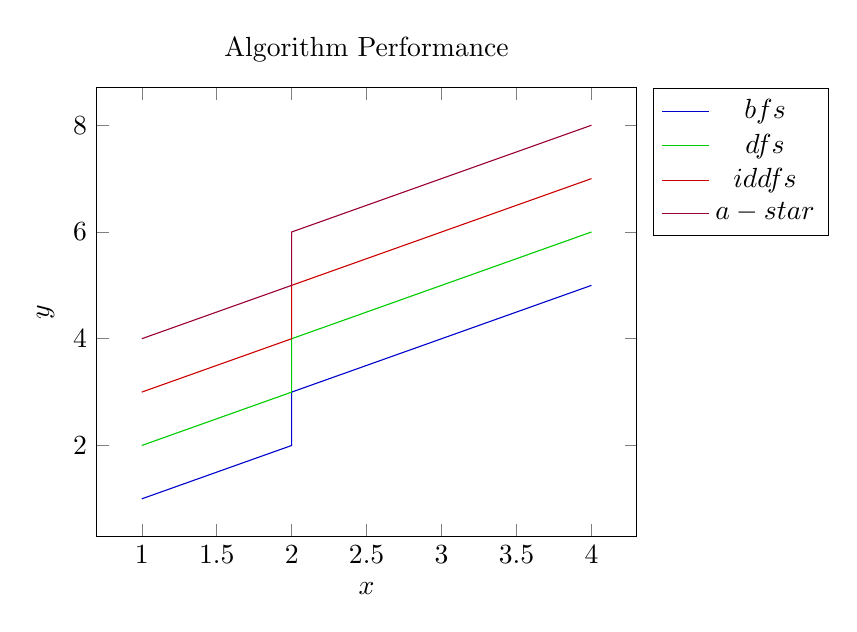
\begin{tikzpicture}
      \begin{axis}[
        title=Algorithm Performance,
        legend pos=outer north east,
        xlabel=$x$,
        ylabel={$y$}
        ]
        \addplot[blue!80!black]
          coordinates
          {(1,1)(2,2)(2,3)(3,4)(4,5)};
        \addplot[green!80!black]
          coordinates
          {(1,2)(2,3)(2,4)(3,5)(4,6)};
        \addplot[red!80!black]
          coordinates
          {(1,3)(2,4)(2,5)(3,6)(4,7)};
        \addplot[purple!80!black]
          coordinates
          {(1,4)(2,5)(2,6)(3,7)(4,8)};
          \legend{{$bfs$},{$dfs$},{$iddfs$},{$a-star$}}
        \end{axis}
    \end{tikzpicture}
  \end{center}

  \subsection{Discussion}
  \subsection{Conclusion}
\end{document}
